%============================================================================%
%
%	DOCUMENT DEFINITION
%
%============================================================================%

\input{glyphtounicode}
\pdfgentounicode=1

%we use article class because we want to fully customize the page and don't use a cv template
\documentclass[10pt,A4]{article}	


%----------------------------------------------------------------------------------------
%	ENCODING
%----------------------------------------------------------------------------------------

% we use utf8 since we want to build from any machine
\usepackage[utf8]{inputenc}		

%----------------------------------------------------------------------------------------
%	LOGIC
%----------------------------------------------------------------------------------------

% provides \isempty test
\usepackage{xstring, xifthen}

%----------------------------------------------------------------------------------------
%	FONT BASICS
%----------------------------------------------------------------------------------------

% some tex-live fonts - choose your own

%\usepackage[defaultsans]{droidsans}
%\usepackage[default]{comfortaa}
%\usepackage{cmbright}
\usepackage[default]{raleway}
%\usepackage{fetamont}
%\usepackage[default]{gillius}
%\usepackage[light,math]{iwona}
%\usepackage[thin]{roboto} 

% set font default
\renewcommand*\familydefault{\sfdefault} 	
\usepackage[T1]{fontenc}

% more font size definitions
\usepackage{moresize}

%----------------------------------------------------------------------------------------
%	FONT AWESOME ICONS
%---------------------------------------------------------------------------------------- 

% include the fontawesome icon set
\usepackage{fontawesome}

% use to vertically center content
% credits to: http://tex.stackexchange.com/questions/7219/how-to-vertically-center-two-images-next-to-each-other
\newcommand{\vcenteredinclude}[1]{\begingroup
\setbox0=\hbox{\includegraphics{#1}}%
\parbox{\wd0}{\box0}\endgroup}

% use to vertically center content
% credits to: http://tex.stackexchange.com/questions/7219/how-to-vertically-center-two-images-next-to-each-other
\newcommand*{\vcenteredhbox}[1]{\begingroup
\setbox0=\hbox{#1}\parbox{\wd0}{\box0}\endgroup}

% icon shortcut
\newcommand{\icon}[3] { 							
	\makebox(#2, #2){\textcolor{maincol}{\csname fa#1\endcsname}}
}	

% icon with text shortcut
\newcommand{\icontext}[4]{ 						
	\vcenteredhbox{\icon{#1}{#2}{#3}}  \hspace{2pt}  \parbox{0.9\mpwidth}{\textcolor{#4}{#3}}
}

% icon with website url
\newcommand{\iconhref}[5]{ 						
    \vcenteredhbox{\icon{#1}{#2}{#5}}  \hspace{2pt} \href{#4}{\textcolor{#5}{#3}}
}

% icon with email link
\newcommand{\iconemail}[5]{ 						
    \vcenteredhbox{\icon{#1}{#2}{#5}}  \hspace{2pt} \href{mailto:#4}{\textcolor{#5}{#3}}
}

\newcommand{\iconegithub}[5]{                         
    \vcenteredhbox{\icon{#1}{#2}{#5}}  \hspace{2pt} \href{#4}{\textcolor{#5}{#3}}
}


%----------------------------------------------------------------------------------------
%	PAGE LAYOUT  DEFINITIONS
%----------------------------------------------------------------------------------------

% page outer frames (debug-only)
% \usepackage{showframe}		

% we use paracol to display breakable two columns
\usepackage{paracol}

% define page styles using geometry
\usepackage[a4paper]{geometry}

% remove all possible margins
\geometry{top=1cm, bottom=1cm, left=1cm, right=1cm}

\usepackage{fancyhdr}
\pagestyle{empty}

% space between header and content
% \setlength{\headheight}{0pt}

% indentation is zero
\setlength{\parindent}{0mm}

%----------------------------------------------------------------------------------------
%	TABLE /ARRAY DEFINITIONS
%---------------------------------------------------------------------------------------- 

% extended aligning of tabular cells
\usepackage{array}

% custom column right-align with fixed width
% use like p{size} but via x{size}
\newcolumntype{x}[1]{%
>{\raggedleft\hspace{0pt}}p{#1}}%


%----------------------------------------------------------------------------------------
%	GRAPHICS DEFINITIONS
%---------------------------------------------------------------------------------------- 

%for header image
\usepackage{graphicx}

% use this for floating figures
% \usepackage{wrapfig}
% \usepackage{float}
% \floatstyle{boxed} 
% \restylefloat{figure}

%for drawing graphics		
\usepackage{tikz}				
\usetikzlibrary{shapes, backgrounds,mindmap, trees}

%----------------------------------------------------------------------------------------
%	Color DEFINITIONS
%---------------------------------------------------------------------------------------- 
\usepackage{transparent}
\usepackage{color}

% primary color
\definecolor{maincol}{RGB}{ 0, 36, 88 }

% accent color, secondary
% \definecolor{accentcol}{RGB}{ 250, 150, 10 }

% dark color
\definecolor{darkcol}{RGB}{ 70, 70, 70 }

% light color
\definecolor{lightcol}{RGB}{220,220,220}


% Package for links, must be the last package used
\usepackage[hidelinks]{hyperref}

% returns minipage width minus two times \fboxsep
% to keep padding included in width calculations
% can also be used for other boxes / environments
\newcommand{\mpwidth}{\linewidth-\fboxsep-\fboxsep}
	


%============================================================================%
%
%	CV COMMANDS
%
%============================================================================%

%----------------------------------------------------------------------------------------
%	 CV LIST
%----------------------------------------------------------------------------------------

% renders a standard latex list but abstracts away the environment definition (begin/end)
\newcommand{\cvlist}[1] {
	\begin{itemize}{#1}\end{itemize}
}

%----------------------------------------------------------------------------------------
%	 CV TEXT
%----------------------------------------------------------------------------------------

% base class to wrap any text based stuff here. Renders like a paragraph.
% Allows complex commands to be passed, too.
% param 1: *any
\newcommand{\cvtext}[1] {
	\begin{tabular*}{1\mpwidth}{p{0.98\mpwidth}}
		\parbox{1\mpwidth}{#1}
	\end{tabular*}
}

%----------------------------------------------------------------------------------------
%	CV SECTION
%----------------------------------------------------------------------------------------

% Renders a a CV section headline with a nice underline in main color.
% param 1: section title
\newcommand{\cvsection}[1] {
	\vspace{4pt}
	\cvtext{
		\textbf{\LARGE{\textcolor{darkcol}{#1}}}\\[-4pt]
		\textcolor{maincol}{ \rule{0.1\textwidth}{2pt} } \\
	}
}

%----------------------------------------------------------------------------------------
%	META SKILL
%----------------------------------------------------------------------------------------

% Renders a progress-bar to indicate a certain skill in percent.
% param 1: name of the skill / tech / etc.
% param 2: level (for example in years)
% param 3: percent, values range from 0 to 1
\newcommand{\cvskill}[3] {
	\begin{tabular*}{1\mpwidth}{p{0.72\mpwidth}  r}
 		\raggedright\textcolor{black}{\textbf{#1}} & \textcolor{maincol}{#2}\\
	\end{tabular*}%
	
	\hspace{4pt}
	\begin{tikzpicture}[scale=1,rounded corners=2pt,very thin]
		\fill [lightcol] (0,0) rectangle (1\mpwidth, 0.1);
		\fill [maincol] (0,0) rectangle (#3\mpwidth, 0.1);
  	\end{tikzpicture}%
}

\newcommand{\cvskillcompact}[3] {
	\begin{tabular*}{1\mpwidth}{p{0.72\mpwidth}  r}
 		\raggedright\textcolor{black}{\textbf{#1}} & \textcolor{maincol}{#2}\\
	\end{tabular*}%
	
	\hspace{4pt}
	\begin{tikzpicture}[scale=1,rounded corners=2pt,very thin]
		\fill [lightcol] (0,0) rectangle (1\mpwidth, 0.1);
		\fill [maincol] (0,0) rectangle (#3\mpwidth, 0.1);
  	\end{tikzpicture}%
}

%----------------------------------------------------------------------------------------
%	 CV EVENT
%----------------------------------------------------------------------------------------

% Renders a table and a paragraph (cvtext) wrapped in a parbox (to ensure minimum content
% is glued together when a pagebreak appears).
% Additional Information can be passed in text or list form (or other environments).
% the work you did
% param 1: time-frame i.e. Sep 14 - Jan 15 etc.
% param 2:	 event name (job position etc.)
% param 3: Customer, Employer, Industry
% param 4: Short description
% param 5: work done (optional)
% param 6: technologies include (optional)
% param 7: achievements (optional)
\newcommand{\cvevent}[7] {
	
	% we wrap this part in a parbox, so title and description are not separated on a pagebreak
	% if you need more control on page breaks, remove the parbox
    % \parbox{\mpwidth}{
    %     \begin{tabular*}{1\mpwidth}{@{} p{\dimexpr0.59\mpwidth-\tabcolsep} r @{}}
    %         \textcolor{black}{\textbf{#2}} & \colorbox{maincol}{\makebox[0.42\mpwidth]{\textcolor{white}{#1}}} \\
    %         \textcolor{maincol}{\textbf{#3}} & \\
    %     \end{tabular*}\\[8pt]

    %     \ifthenelse{\isempty{#4}}{}{
    %         \cvtext{#4}
    %     }
    % }
    \parbox{\mpwidth}{
      \begin{tabular*}{1\mpwidth}{p{0.59\mpwidth}  r}
          \textcolor{black}{\large{\textbf{#2}}} & \colorbox{white}{\makebox[0.52\mpwidth]{\textcolor{black}{#1}}} \\
          \textcolor{maincol}{\textbf{#3}} & \\
      \end{tabular*}\\[0pt]
    
      \ifthenelse{\isempty{#4}}{}{
          \cvtext{#4}
      }
    }    
	% \parbox{\mpwidth}{
    %   \begin{tabular*}{1\mpwidth}{p{0.59\mpwidth}  r}
    %       \textcolor{black}{\textbf{#2}} & \colorbox{white}{\makebox[0.42\mpwidth]{\textcolor{black}{#1}}} \\
    %       \textcolor{maincol}{\textbf{#3}} & \\
    %   \end{tabular*}\\[8pt]
    
    %   \ifthenelse{\isempty{#4}}{}{
    %       \cvtext{#4}
    %   }
    % } 

	\ifthenelse{\isempty{#5}}{}{
		\vspace{0pt}
		{#5}
	}

	\ifthenelse{\isempty{#6}}{}{
		\vspace{0pt}
		\cvtext{\textbf{Technologies:}}
		{#6}
	}

	\ifthenelse{\isempty{#7}}{}{
		\vspace{4pt}
		\cvtext{\textbf{Achievements:}}
		{#7}
	}
	\vspace{12pt}
}

%----------------------------------------------------------------------------------------
%	 CV META EVENT
%----------------------------------------------------------------------------------------

% Renders a CV event on the sidebar
% param 1: title
% param 2: subtitle (optional)
% param 3: customer, employer, etc,. (optional)
% param 4: info text (optional)
\newcommand{\cvmetaevent}[4] {


	\ifthenelse{\isempty{#2}}{}{
	\textcolor{darkcol} {\cvtext{\textbf{#2}} }
	}

	\ifthenelse{\isempty{#3}}{}{
		\cvtext{{ \textcolor{darkcol} {#3} }}\\
	}

	\cvtext{#4}\\[14pt]
}

%---------------------------------------------------------------------------------------
%	QR CODE
%----------------------------------------------------------------------------------------

% Renders a qrcode image (centered, relative to the parentwidth)
% param 1: percent width, from 0 to 1
\newcommand{\cvqrcode}[1] {
	\begin{center}
		
\includegraphics[width={#1}\mpwidth]{qrcode}
	\end{center}
}


%============================================================================%

%%
%
%	DOCUMENT CONTENT
%
%
%
%============================================================================%
\begin{document}
\columnratio{0.31}
\setlength{\columnsep}{2.2em
}\setlength{\columnseprule}{3pt}
\colseprulecolor{lightcol}
\begin{paracol}{2}
\begin{leftcolumn}
%---------------------------------------------------------------------------------------
%	META IMAGE + info
%----------------------------------------------------------------------------------------
%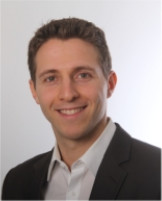
\includegraphics[width=\linewidth]{untitled.jpg}	%trimming relative to image size



\vfill\null
\cvsection{Contact}
	
\icontext{MapMarker}{12}{Puy de Merland\\24110 St Astier, France}{black}\\[4pt]
\icontext{MobilePhone}{12}{+33 6 75 10 87 20}{black}\\[4pt]
\iconemail{Envelope}{12}{ha.lagrange9000@gmail.com}{ha.lagrange9000@gmail.com}{black}\\[4pt]
\iconegithub{Github}{12}{github.com/Dedalum}{https://github.com/Dedalum}{black}\\


%---------------------------------------------------------------------------------------
%	META SKILLS
%----------------------------------------------------------------------------------------
\cvsection{Compétences}

\begin{tabular*}{1\linewidth}{p{0.18\linewidth} >{\raggedright\arraybackslash}p{0.75\linewidth}}
	\textcolor{black}{\LARGE{+++}} & \textcolor{black}{Python, Bash, git }\\[5pt]
	\textcolor{black}{\LARGE{++}} & \textcolor{black}{Golang, SQL, Ansible, InfluxDB/Grafana, ELK stack, AWS/GCP, VPC, routage}\\[5pt]
	\textcolor{black}{\LARGE{+}} & \textcolor{black}{Tailwind, Nuxt/Vue, Jenkins, K8s, Terraform}\\[5pt]
	\textcolor{black}{\textbf{Other}} & \textcolor{black}{Méthodes Agile: Scrum \& Kanban, communication pluridisciplinaire, support client, bases marketing}\\[5pt]  
\end{tabular*}%

\cvsection{Langues}

\begin{tabular*}{1\linewidth}{p{0.33\linewidth} >{\raggedright\arraybackslash}p{0.67\linewidth}}
	\textcolor{black}{\textbf{Bilingue}} & \textbf{\textcolor{black}{Anglais, Français}}\\[5pt]  
	\textcolor{black}{\textbf{A2/à l'étude}} & \textcolor{black}{Allemand, suédois, espagnol}\\[5pt]
\end{tabular*}%


%---------------------------------------------------------------------------------------
%	EDUCATION
%----------------------------------------------------------------------------------------
\cvsection{Éducation}

\cvmetaevent
{}
{Master, réseaux et informatique}
{Université de Technologie de Troyes \\Troyes, France, 2011 - 2016}
{Réseaux et informatique, spécialité en sécurité de l'information: mathématiques, télécoms,
traitement d'image et cryptographie, infosec, réseaux (routeurs, VPC, Cisco)}

% -------
% Extra
% -------

\cvsection{Intérêts}
{\cvlist{
    \item Techno crypto/blockchaîne,\\infosec, IoT, applications IA
    \item Business \& marketing \& startups, questions environnementales \& énergétiques
    \item Littérature, brassage de bière, randonnées
}}

%---------------------------------------------------------------------------------------
%	CERTIFICATION
%----------------------------------------------------------------------------------------
% \newpage
% \cvsection{CERTIFICATIONS}

% \cvmetaevent
% {LPIC 1 - Linux administrator}
% {}
% {}
% {Certificate issued by the Linux Professional Institute to prove abilities in Linux administration}


\end{leftcolumn}
\begin{rightcolumn}
%---------------------------------------------------------------------------------------
%	TITLE  HEADER
%----------------------------------------------------------------------------------------
\fcolorbox{white}{white}{\begin{minipage}[c][1cm][c]{1\mpwidth}
	\begin {center}
		\textbf{ \Large{ \textcolor{black}{ Hugues Lagrange } }  | \large{ \textcolor{black} {Développeur} } }
	\end {center}
\end{minipage}} \\[1pt]
\vspace{-6pt}

%---------------------------------------------------------------------------------------
%	PROFILE
%----------------------------------------------------------------------------------------
\cvtext{À la recherche de challenges, de produits intéressants et d'esprit d'équipe. Développeur avec une expérience spécifique en Python et en Golang qui s'intéresse aux startups et marketing. J'aime automatiser les choses et prendre les problèmes à bras-le-corps.
}\\[8pt]

%---------------------------------------------------------------------------------------
%	WORK EXPERIENCE
%----------------------------------------------------------------------------------------
\cvsection{Expérience professionnelle}
\cvevent
    {11/23 - en cours}
    {Projet personnel/professionnel}
    {\href{https://maitre-hanguk.com}{Maître Hanguk}}
    {Développement d'un site pour apprendre le coréen, avec future évolution payante. \\[4pt]
    Technos: FastAPI, Nuxt 3/Vue 3, Tailwind, Postgres, Ansible, Traefik, Web marketing \& SEO}
    {}
    {}
    {}
\cvevent
    {02/23 - 05/23, 4 mois}
    {Projet professionnel: développement d'une SaaS}
    {PDF Toolkit API - Remote, France}
    {Développement d'une SaaS offrant une API pour générer divers types de documents PDF (reçus, rapports, CV) dans une équipe de 2 personnes. \\[4pt]
    Technos: FastAPI, Vue 3, Tailwind, Postgres, Ansible, Traefik, Web marketing \& SEO}
    {}
    {}
    {}

\cvevent
	{04/20 - 07/23, 3 ans 4 m}
	{Développeur Python}
	{Linxo Group - Télétravail /Aix-en-Provence, France}
	{Linxo est une startup française dans la fintech qui agrège des données bancaires et financières pour des individus et des entreprises. \\
    J'étais membre de l'équipe responsable de l'agrégation des données et leur gestion pour pré-analyse dans un environnement soumis aux RGPD.}
    {\cvlist{
        \item Design et implémentation de features et logique business en équipes transverses pour l'agrégation de données bancaires et financières
        \item Support N3, relations directes avec des clients et banques françaises
        \item \textbf{Technologies:} Python, PostgreSQL, Java/Go, Jenkins, ELK stack, métriques Grafana (Postgres, Influxdb), Bash
    }}
    {}
    {}

% \vfill\null
\cvevent
	{05/17 - 08/18, 1 an 4 m}
    {Développeur Golang \& Python}
    {Snuk - Berlin, Allemagne}
    {Jeune startup dans l'internet des objets: développement d'une infrastructure pour "bâtiments intelligents".}
    {\cvlist{
        \item Design de systèmes distribués, implémentation et installation sur site \\
        d'infrastructures IoT et architectures cloud
        \item Développement produit avec les clients et support à distance et sur site de l'infrastructure
        \item \textbf{Technologies:} Golang \& Python, Bash, Postgres, MongoDB, GCP, Docker, Ansible, TIGK stack, IoT (BLE, MQTT, Raspberry Pi)
    }}
    {}
    {}

% \vfill\null
\cvevent
    {03/16 - 09/16, 6 mois}
    {Stage devops/securité info}
    {Freespee AB - Uppsala, Suède}
    {Freespee est une SaaS de marketing. Technlogoies: AWS, stack ELK \& Redis, Ansible, serveur OpenVPN, Linux, Bash \& scripts Python.}
    % I worked as an intern in the engineering team, in Uppsala, Sweden, performing system administration tasks with a focus on information security. Along my different projects were}
    % {\cvlist{
    %     \item Deploying an ELK stack for central log management with a Redis buffer in an AWS VPC (25 VMs)
    %     \item Preparing an office firewall based on Debian (iptables scripts, Suricata IDS, OpenVPN bridge, VLANs, DHCP and local DNS)
    %     \item Installing an OpenVPN server for a secure remote access to the AWS VPC
    %     \item Research and setup of a ”chatops” solution using Slack and Errbot, Jenkins, Ansible and Docker 
    % }}
	{}
    {}
	{}

% \vfill\null
\cvevent
    {02/15 - 07/15, 6 mois}
	{Administrateur système}
    {Jymeo - Nantes, France}
    {JYMEO offre un service de comparaison de prix de pneus et autres. Technologies: cloud OVH, stack ELK, Ansible, serveur OpenVPN, Linux, Bash \& scripting Python.}
    % We followed the Scrum method. I deployed and worked on the ELK suite for analyzing server logs, deployed OpenVPN servers and backup scripts, firewalls (iptables, fail2ban, NAXSI), secured Wordpress websites.}
    % {\cvlist{
    %     \item Setting up new servers (Virtual machines running Debian 8, with providers OVH/RunAbove) with web-servers (Nginx, Apache)
    %     \item Level 3 support
    % }}
    {}
    {}
    {}

% hotfixes to create fake-space to ensure the whole height is used
% \mbox{}
% \vfill
% \mbox{}
% \vfill
% \mbox{}
% \vfill
% \mbox{}
\end{rightcolumn}
\end{paracol}
\end{document}

